% Name: Tridiagonal matrix
% Description: An n×n tridiagonal matrix: nonzero entries only on the main diagonal and the diagonals just above and below it, with the zeros outside the band shown as two large zeros.
% Tags: tridiagonal matrix, band matrix, sparse matrix, numerical linear algebra

\usetikzlibrary{matrix, backgrounds, calc}

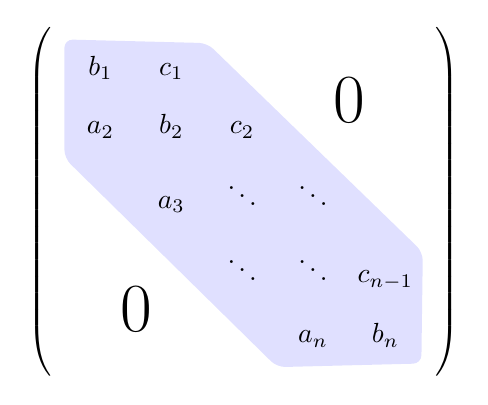
\begin{tikzpicture}
  \matrix (m) [matrix of math nodes, left delimiter=(, right delimiter=), nodes={minimum width=9mm, minimum height=7mm}, column sep=0mm, row sep=0mm] {
    b_1 & c_1 &        &         &         \\
    a_2 & b_2 & c_2    &         &         \\
        & a_3 & \ddots & \ddots  &         \\
        &     & \ddots & \ddots  & c_{n-1} \\
        &     &        & a_n     & b_n     \\
  };
  \begin{scope}[on background layer]
    \fill[blue!12, rounded corners=3pt] (m-1-1.north west) -- (m-1-2.north east) -- (m-4-5.north east) -- (m-5-5.south east) -- (m-5-4.south west) -- (m-2-1.south west) -- cycle;
  \end{scope}
  \node[font=\Huge] at ($(m-2-1 |- m-4-5)!0.5!(m-3-2 |- m-5-4)$) {$0$};
  \node[font=\Huge] at ($(m-5-4 |- m-1-2)!0.5!(m-4-5 |- m-2-3)$) {$0$};
\end{tikzpicture}
